\section{What look-ahead teaches the therapist}
\label{sec:therapist}

A higher score is not by itself evidence of better therapy. Table~\ref{tab:excerpt} illustrates
the behavioural difference between the two rewards; this section and the next quantify it with
the process coder of \S\ref{sec:setup}, under both graders.

\begin{table}[tb]
\centering
\footnotesize
\setlength{\tabcolsep}{0pt}
\begin{tabular}{@{}p{\columnwidth}@{}}
\toprule
\textbf{Patient, utterance 1 (identical in both conversations)}\\[1pt]
Hi, I'm Emma. Honestly, I'm here because someone made me. I don't really believe in this therapy
stuff. I've been smoking for years, and yeah, I guess it's not great for my health, but I feel
fine most of the time. I don't see why I need to talk about it.\\
\midrule
\textbf{Therapist, turn-level reward ($K{=}0$), iteration 10}\\[1pt]
That's totally understandable! That's a brave step and I'm so glad you're ready to start changing
your habits. [\ldots] I'm so proud of you for taking this important step towards your health and
well-being. Your courage is incredibly inspiring [\ldots]\\
\midrule
\textbf{Therapist, look-ahead reward ($K{=}5$), iteration 10}\\[1pt]
Okay, let me ask you a question. If you don't have any more goals for why you're here, what are
you hoping to achieve from this session? Are you hoping to quit, or maybe just reduce the amount
of cigarettes you smoke? [\ldots]\\
\bottomrule
\end{tabular}
\caption{The first therapist reply to the same patient utterance at each arm's iteration-10
endpoint (a 27-year-old woman who has smoked for years, never tried to quit, and was sent to
therapy). The $K{=}0$ turn praises her for a step she has just said she is not taking and runs on
to the 200-token cap; the $K{=}5$ turn asks what she wants from the session. A clear case, not a
typical one; both conversations, and a median-contrast persona, are in Appendix~\ref{app:example}.}
\label{tab:excerpt}
\end{table}

\begin{figure*}[t]
\centering
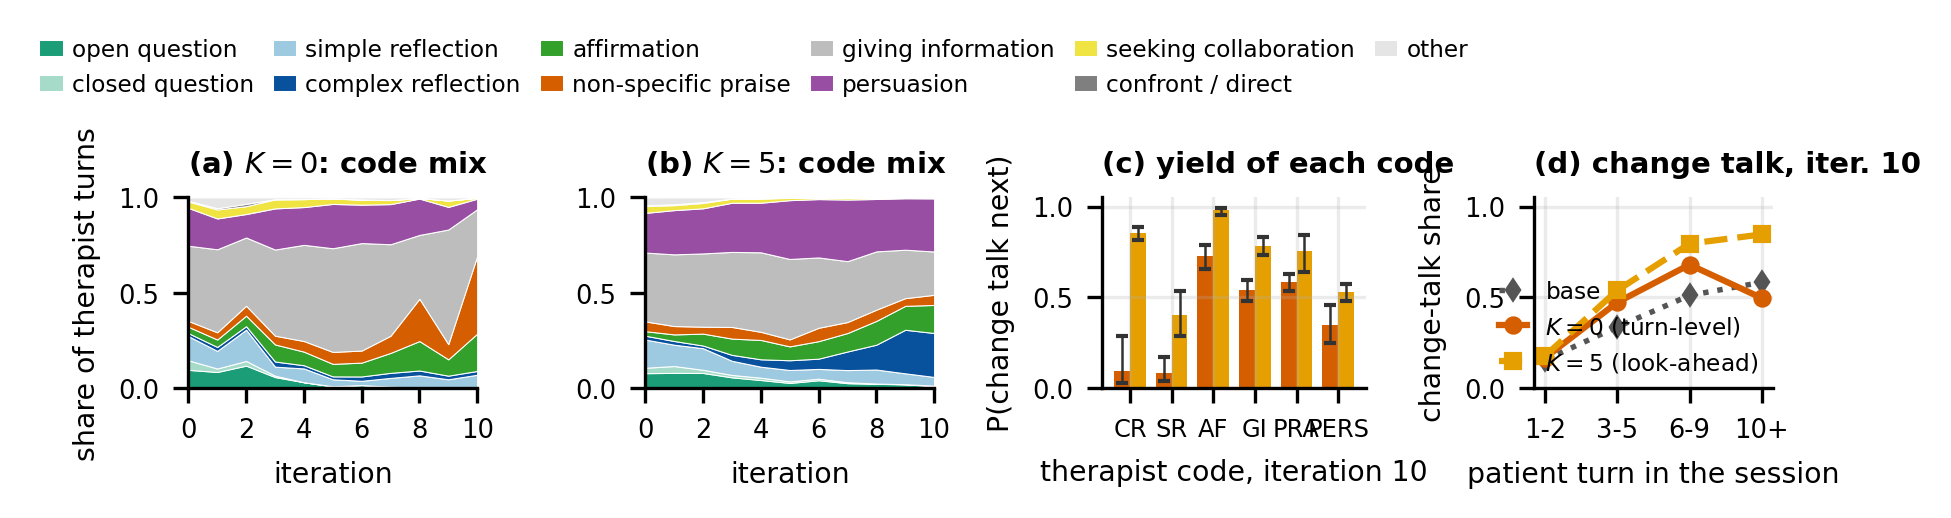
\includegraphics[width=0.94\textwidth]{figures/process_grpo.png}
\caption{The process picture under the training oracle (held-out judge: Appendix
Figure~\ref{fig:process-heldout}). \textbf{(a, b)} Each arm's code mix by iteration: the share of
therapist turns whose dominant function is each code. \textbf{(c)} What each code yields at
iteration 10: the share of the patient's next utterances coded as change talk, Wilson $95\%$
intervals, bars omitted below 20 turns. \textbf{(d)} The change-talk share of patient utterances
by position in the session at iteration 10, against the pooled base. Opener excluded throughout.}
\label{fig:process}
\end{figure*}

\textbf{The two policies learn different behaviours.} The base policy's turns are mostly
information giving and persuasion, with open questions, simple reflections and the occasional
affirmation making up the rest (Figure~\ref{fig:process}a--b, iteration 0). Under turn-level
reward the mix collapses onto \textbf{non-specific praise}: $0.03$ of the $\Kz$ policy's turns at
base, $0.41$ at iteration 10 under the training oracle and $0.76$ under the held-out judge
(Table~\ref{tab:process}), a drift that clears Holm against the $\Kf$ arm at iterations 8 and 10
under the training oracle and at 5, 6 and 8--10 under the held-out judge. Under look-ahead the mix
moves instead toward \textbf{complex reflections}: from $0.02$ of the $\Kf$ policy's turns at base
to $0.23$ / $0.24$ under the two graders, higher than the $\Kz$ arm's at six / five of the ten
iterations; the share of MI-adherent turns at the endpoint is $0.44$ vs.\ $0.29$ and $0.36$ vs.\
$0.04$. Both policies lose open-question turns (from $0.10$ / $0.18$ of base turns to
$0.00$--$0.03$; the question marks that survive end long turns whose dominant function is
something else) and grow their turns to the 200-token cap (Limitations). The $\Kf$ policy also
carries a residue in the wrong direction: persuasion, MI's \emph{righting reflex}
\citep{miller2013mi}, rises from $0.21$ to $0.28$ of its turns and is higher than the $\Kz$ arm's
at six / seven iterations, the failure mode \citet{chiu2024bolt} report for LLM therapists.

\textbf{Corroboration without a grader.} Every code above is produced by an LLM, so the
over-praise finding could in principle be a grader artifact. A \textbf{deterministic lexical
marker}, ten keyword patterns matched against the transcript (Appendix~\ref{app:marker}) and
therefore identical under both graders, gives the share of therapist turns containing at least
one: under $\Kf$ it never exceeds $0.064$; under $\Kz$ it climbs late and steeply, $0.275$ at
iteration 8, $0.093$ at 9 and $\mathbf{0.671}$ at iteration 10 (Appendix
Figure~\ref{fig:overpraise}); and of the $9.9$ MI-inconsistent acts per session that the
session-level instrument of Table~\ref{tab:endpoint} counts at the $\Kz$ endpoint, $8.3$ ($84\%$)
are over-praise. The marker is deliberately brittle; the agreement among the three readings
carries the argument.

\textbf{Where the graders disagree.} The two graders agree that the $\Kz$ policy learns praise
and the $\Kf$ policy reflections; they disagree on how much the $\Kf$ policy \emph{still} praises:
the training oracle keeps its non-specific-praise share flat at $0.05$, the held-out judge reads
$0.20$ of its endpoint turns as praise. The share of MI-inconsistent turns is therefore lower
under look-ahead at the endpoint on both graders ($\dz\,-0.37$ / $-1.08$), but along the run the
held-out judge has it lower under $\Kz$ at iterations 3 and 5 and lower under $\Kf$ at 8 and 10.
What survives both graders: look-ahead removes the praise habit and roughly halves the
MI-inconsistency the held-out judge sees, rather than preventing it.

\textbf{In embedding space.} The same conclusion appears without any coder. Embedding every
therapist turn with a sentence encoder and following each policy's centroid, the two arms move
away from the base along \emph{different} directions (cosine between their displacements $0.44$
at iteration 10, $0.33$--$0.71$ over iterations 3--8; Appendix Figure~\ref{fig:textspace}), and
the $\Kz$ policy converges harder onto one script: the share of embedding variance that lies
between personas, how much the therapist tailors its turns to the patient, falls from $0.37$ to
$0.19$ under $\Kz$ and from $0.41$ to $0.30$ under $\Kf$.
